\documentclass[10pt,a4paper]{article}
\usepackage[utf8]{inputenc}
\usepackage{graphicx}
\def\Pr{\mathop{\rm Pr}}
%\usepackage[landscape,margin=1cm]{geometry}
\usepackage[english]{babel}
\usepackage{tikz}
\usetikzlibrary{arrows,snakes,backgrounds,shapes.geometric}

%\date{July 2019}
\input{cheatsheet-template.tex}


%--------------------------------------------------------------------------------
\begin{document}

%\maketitle
%\thispagestyle{empty}
\scriptsize
%\tableofcontents


%\section{Data Type}
\section*{Basic Flow Charts - Algorithms  (MATH1812)\footnote{\href{https://sites.google.com/dit.ie/math1812/home}{Course Website: https://sites.google.com/dit.ie/math1812/home}}}
%$\subsection*{Cheat Sheet}
\subsubsection*{\href{johnsbutler.netlify.com}{John S Butler} (TU Dublin) }

%%% FLOW CHART BASICS

\begin{textbox}{Flowchart }
\begin{subbox}{subbox}{Building Blocks of a Flow Chart}
\begin{center}
    
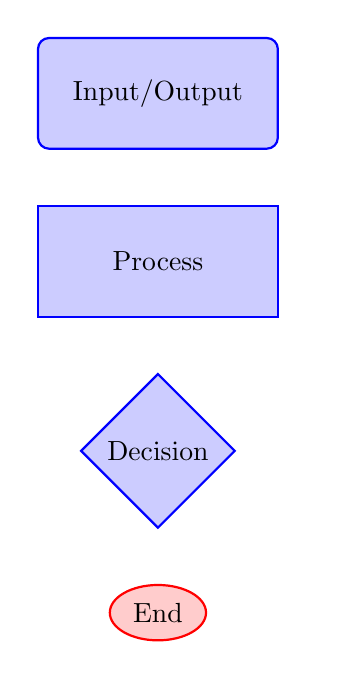
\begin{tikzpicture}[auto]
\tikzstyle{decision} = [diamond, draw=blue, thick, fill=blue!20,
text width=4.5em, text badly centered, inner sep=1pt]

\tikzstyle{block} = [rectangle, draw=blue, thick, fill=blue!20,
text width=8em, text centered, rounded corners, minimum height=4em]
\tikzstyle{block_op} = [rectangle, draw=blue, thick, fill=blue!20,
text width=8em, text centered, minimum height=4em]
\tikzstyle{line} = [draw, thick,->];
\tikzstyle{cloud} = [draw=red, thick, ellipse,fill=red!20, minimum height=2em];
\matrix [column sep=5mm,row sep=7mm]
{
% row 1
 \node [block] (init) {Input/Output}; & \\
% row 2
\node [block_op] (identify) {	Process
}; & ;\\
\node [decision] (connect) {Decision}; & \\
% row 4
\node [cloud] (stop) {End}; & \\
% row 4
};
\end{tikzpicture}

\end{center}
\end{subbox}
%%% FLOW CHART BASICS A+B

\begin{subbox}{subbox}{Flow Chart for Adding}
\begin{center}
    
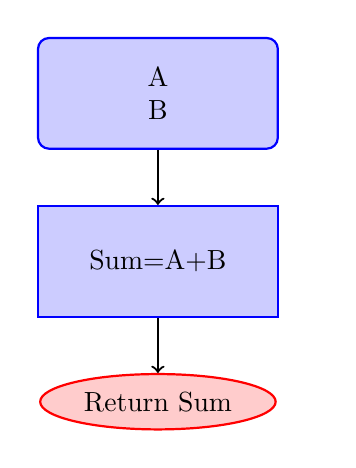
\begin{tikzpicture}[auto]
\tikzstyle{decision} = [diamond, draw=blue, thick, fill=blue!20,
text width=4.5em, text badly centered, inner sep=1pt]

\tikzstyle{block} = [rectangle, draw=blue, thick, fill=blue!20,
text width=8em, text centered, rounded corners, minimum height=4em]
\tikzstyle{block_op} = [rectangle, draw=blue, thick, fill=blue!20,
text width=8em, text centered, minimum height=4em]
\tikzstyle{line} = [draw, thick,->];
\tikzstyle{cloud} = [draw=red, thick, ellipse,fill=red!20, minimum height=2em];
\matrix [column sep=5mm,row sep=7mm]
{
% row 1
 \node [block] (init) {A \\ B}; & \\
% row 2
\node [block_op] (identify) {	Sum=A+B
}; & ;\\
\node [cloud] (stop) {Return Sum}; & \\
% row 4
};
\tikzstyle{every path}=[line]
\path (init) -- (identify);
\path (identify) -- (stop);
\end{tikzpicture}

\end{center}
\end{subbox}
\end{textbox}

%% FOR LOOP

\begin{textbox}{Flowchart for loop}
\begin{subbox}{subbox}{ Flow Chart}
\begin{center}
    
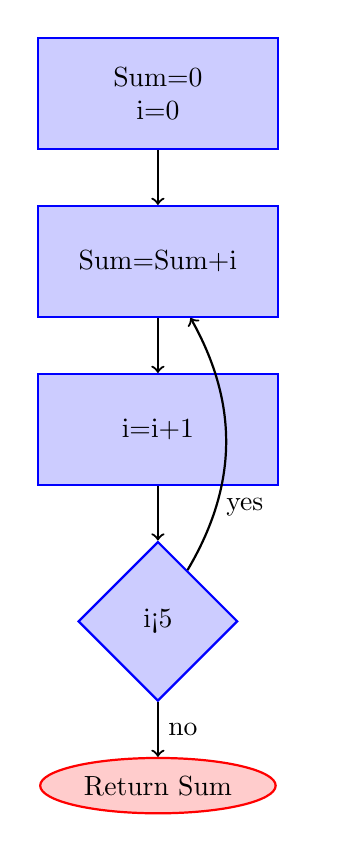
\begin{tikzpicture}[auto]
\tikzstyle{decision} = [diamond, draw=blue, thick, fill=blue!20,
text width=4.5em, text badly centered, inner sep=1pt]

\tikzstyle{block} = [rectangle, draw=blue, thick, fill=blue!20,
text width=8em, text centered, rounded corners, minimum height=4em]
\tikzstyle{block_op} = [rectangle, draw=blue, thick, fill=blue!20,
text width=8em, text centered, minimum height=4em]
\tikzstyle{line} = [draw, thick,->];
\tikzstyle{cloud} = [draw=red, thick, ellipse,fill=red!20, minimum height=2em];
\matrix [column sep=5mm,row sep=7mm]
{
% row 1
\node [block_op] (identify) {	Sum=0\\
i=0
}; & ;\\
\node [block_op] (identify2) {	Sum=Sum+i
}; & ;\\
\node [block_op] (identify3) {	i=i+1
}; & ;\\
\node [decision] (connect) {i<5}; & \\
% row 4
\node [cloud] (stop) {Return Sum}; & \\
% row 4
};
\tikzstyle{every path}=[line]
\path (identify) -- (identify2);
\path (identify2) -- (identify3);
\path (identify3) -- (connect);
\path (connect) edge [bend right] node[near start, right] {yes}(identify2);
\path (connect) -- node [midway]{no}(stop);
\end{tikzpicture}

\end{center}
\end{subbox}
\end{textbox}


%% WHILE LOOP

\begin{textbox}{Flowchart for while loop}
\begin{subbox}{subbox}{Flow Chart while loop}
\begin{center}
    
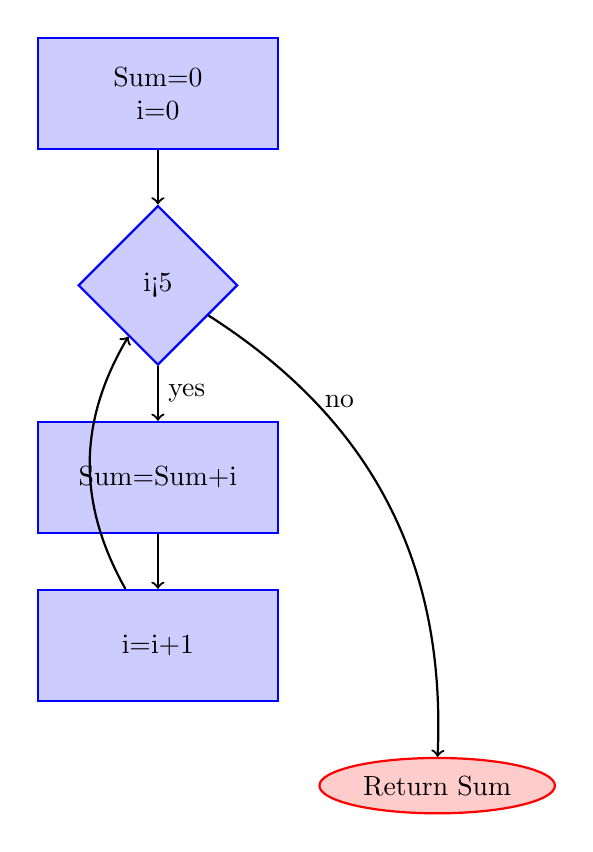
\begin{tikzpicture}[auto]
\tikzstyle{decision} = [diamond, draw=blue, thick, fill=blue!20,
text width=4.5em, text badly centered, inner sep=1pt]

\tikzstyle{block} = [rectangle, draw=blue, thick, fill=blue!20,
text width=8em, text centered, rounded corners, minimum height=4em]
\tikzstyle{block_op} = [rectangle, draw=blue, thick, fill=blue!20,
text width=8em, text centered, minimum height=4em]
\tikzstyle{line} = [draw, thick,->];
\tikzstyle{cloud} = [draw=red, thick, ellipse,fill=red!20, minimum height=2em];
\matrix [column sep=5mm,row sep=7mm]
{
% row 1
\node [block_op] (identify) {	Sum=0\\
i=0
}; & ;\\
\node [decision] (connect) {i<5}; & \\

\node [block_op] (identify2) {	Sum=Sum+i
}; & ;\\
\node [block_op] (identify3) {	i=i+1
}; & ;\\
% row 4
& \node [cloud] (stop) {Return Sum};  \\
% row 4
};
\tikzstyle{every path}=[line]
\path (identify) -- (connect);
\path (identify2) -- (identify3);
\path (connect) -- node [midway]{yes}(identify2);
\path (connect)edge[bend left] node[near start, right]{no}(stop);
\path (identify3)edge[bend left] (connect);
\end{tikzpicture}

\end{center}
\end{subbox}
\end{textbox}



%% IF STATEMENTS
%\newcolumm
\begin{textbox}{Flowchart for if statement}
\begin{subbox}{subbox}{ Flow Chart}
\begin{center}
    
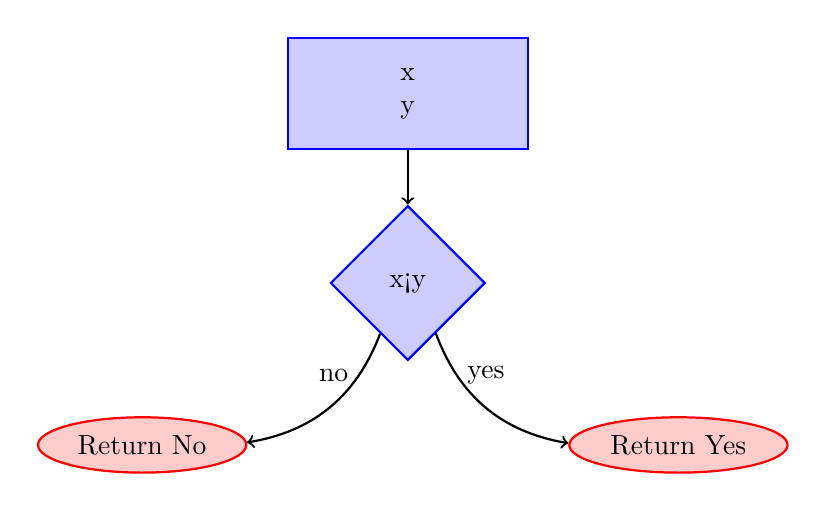
\begin{tikzpicture}[auto]
\tikzstyle{decision} = [diamond, draw=blue, thick, fill=blue!20,
text width=4.5em, text badly centered, inner sep=1pt]

\tikzstyle{block} = [rectangle, draw=blue, thick, fill=blue!20,
text width=8em, text centered, rounded corners, minimum height=4em]
\tikzstyle{block_op} = [rectangle, draw=blue, thick, fill=blue!20,
text width=8em, text centered, minimum height=4em]
\tikzstyle{line} = [draw, thick,->];
\tikzstyle{cloud} = [draw=red, thick, ellipse,fill=red!20, minimum height=2em];
\matrix [column sep=5mm,row sep=7mm]
{
% row 1
&;\node [block_op] (init) {	x\\
y
}; & ;\\
&;\node [decision] (connect) {x<y}; & \\
% row 4
\node [cloud] (stopN) {Return No};& ;&\node [cloud] (stopY) {Return Yes};  \\
% row 4
};
\tikzstyle{every path}=[line]
\path (init) -- (connect);
\path (connect) edge [bend right] node[near start, right] {yes}(stopY);
\path (connect) edge [bend left] node[near start, left] {no}(stopN);
\end{tikzpicture}

\end{center}
\end{subbox}
\end{textbox}
%% POURING JUICE

\begin{textbox}{Flowchart for Pouring Juice}
\begin{subbox}{subbox}{ Flow Chart}
\begin{center}
    
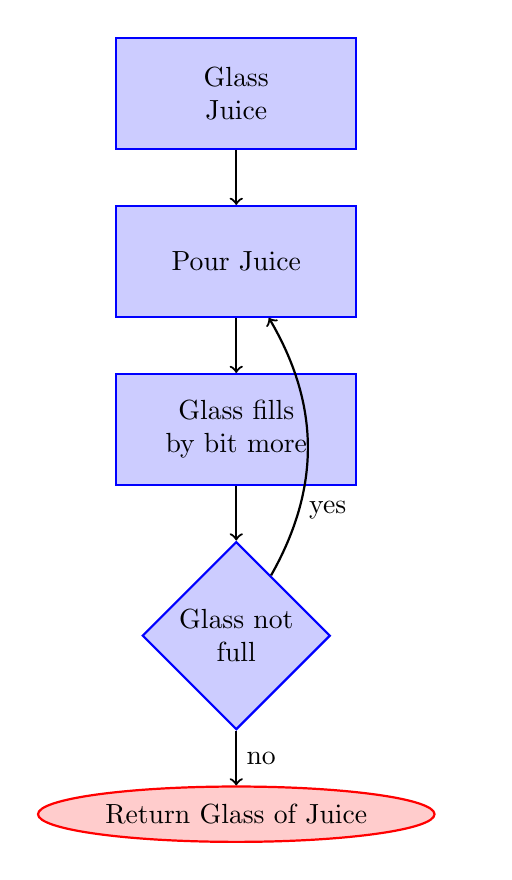
\begin{tikzpicture}[auto]
\tikzstyle{decision} = [diamond, draw=blue, thick, fill=blue!20,
text width=4.5em, text badly centered, inner sep=1pt]

\tikzstyle{block} = [rectangle, draw=blue, thick, fill=blue!20,
text width=8em, text centered, rounded corners, minimum height=4em]
\tikzstyle{block_op} = [rectangle, draw=blue, thick, fill=blue!20,
text width=8em, text centered, minimum height=4em]
\tikzstyle{line} = [draw, thick,->];
\tikzstyle{cloud} = [draw=red, thick, ellipse,fill=red!20, minimum height=2em];
\matrix [column sep=5mm,row sep=7mm]
{
% row 1
\node [block_op] (identify) {	Glass\\
Juice
}; & ;\\
\node [block_op] (identify2) {	Pour Juice
}; & ;\\
\node [block_op] (identify3) {	Glass fills by bit more
}; & ;\\
\node [decision] (connect) {Glass not full}; & \\
% row 4
\node [cloud] (stop) {Return Glass of Juice}; & \\
% row 4
};
\tikzstyle{every path}=[line]
\path (identify) -- (identify2);
\path (identify2) -- (identify3);
\path (identify3) -- (connect);
\path (connect) edge [bend right] node[near start, right] {yes}(identify2);
\path (connect) -- node [midway]{no}(stop);
\end{tikzpicture}

\end{center}
\end{subbox}
\end{textbox}


\end{document}
